\documentclass[hidelinks, 12pt, a4paper]{article}

\usepackage[utf8]{inputenc}
\usepackage[margin=1.5cm]{geometry}
\usepackage{graphicx}
\usepackage{setspace}
\usepackage[T1]{fontenc}
\usepackage{tocloft}
\usepackage{todonotes}
\usepackage{epstopdf} 
\usepackage{hyperref}
\usepackage{float}
\usepackage{titlesec}
\usepackage{listings}
\usepackage{multirow}
\usepackage{xcolor}
\usepackage{mwe}
\usepackage{hyperref}
\onehalfspacing
\usepackage[english]{babel}
\usepackage{fancyhdr}
\usepackage{enumitem}

\pagestyle{fancy}
\fancyhf{}
\rhead{blulancetech@gmail.com}
\lhead{Carpool}
\rfoot{Page \thepage}

\author{}
\date{}
\title
{
	
\includegraphics[width=6cm]{images/up_logo.jpg} \\
	Department of Computer Science \\
	Faculty of Engineering, Built Environment \& IT\\
	University of Pretoria \\
	\vspace{0.5cm}
	\Huge COS301 -
	Software Engineering\\
	\vspace{1cm}
	{\Huge Carpool}\\
	\begin{Large}
		Software Requirements and Design Specifications
	\end{Large}
	\vspace{0.5cm}
	
    \begin{center}
    \noindent
    
\includegraphics[width=6cm]{images/company_logo.png} 
    \vspace{0.5cm}
    \begin{table}[h]
    \centering
    \begin{tabular}{|l|l|l|}
    \hline
    Name  & Student Number\\ \hline
    Benjamin Osmers & u16068344 \\ \hline
    Ashleigh Govender &  U20528834      \\ \hline
    Joshua Brink  & U19185678 \\ \hline
    Jason Antalis     & U19141859     \\ \hline
    Wesley Pachai & U20578688    \\ \hline
            
    \end{tabular}
    \end{table}
    \end{center}
    }
% \setlength {\marginparwidth}{2cm}
\begin{document}
\maketitle


\newpage
\tableofcontents 
\newpage
\section{Project Information}
    
        \qquad \textbf{Project Name:} 
        
           \qquad  \qquad Carpool\\
        
        \textbf{Owner Contact Details:}

          \qquad  \qquad Matthew Wood \qquad \qquad \href{matthew.wood@advance.io}{matthew.wood@advance.io} \qquad \qquad
          
           \qquad  \qquad Keegan Ferrett \qquad \qquad \href{keeganf@mit.edu}{keeganf@mit.edu}\\
           
           
                   \textbf{Lecture mentor:}

          \qquad  \qquad David  \qquad \qquad \href{matthew.wood@advance.io}{matthew.wood@advance.io} \qquad \qquad
          
          	\vspace{1.5cm}
          	
\section{Introduction}
Carpooling is a method of sharing unoccupied seats in a car with people who commute along the same route. Usually, one person from the group drives their personal car and the others all share the cost of the trip. Due to the environmental crisis that the world faces, carpooling has become immensely popular as it reduces the number of cars on the road. Of recent carpooling has become the latest trend as petrol prices continue to increase. Carpooling has evolved into a viable, cost-effective, and stress-free mode of transportation. Finding individuals to carpool with is challenging, since it is difficult to locate someone travelling to the same destination at the same time as you. This Carpool application is a solution to this problem. \\ \\
Carpool is a mobile application that helps students find affordable transport to and from campus or longer trips such as returning home for semester break. Carpool provides students with a central location whereby they can post, find, and join safe car trips. This application allows students with vehicles to save on petrol costs as well as provide affordable transportation to students who do not have vehicles. Students can travel to their desired location while sharing the car and expenditures.\\ \\
\textbf{Vision:}\\
A more affordable and practical version of Uber/Lyft for students. Students can be both drivers and passengers.\\ \\
\textbf{Objective and Scope:} \\
To create an Android and IOS mobile application for students, whereby they are able to post, find and join safe car trips with ease.

\newpage
\section{Users}

\subsection{User Characteristics}
    
The user should have the ability to operate and own a mobile device such as a smartphone or tablet. The user should have constant access to the internet and location services to download and utilize the Carpool application. The following are users of the Carpool System:\\
    
    \Large{ \textbf{Admin} }
    \normalsize
        \begin{itemize}
            \item A person who manages the Carpool system
            \item A person who verifies a user’s email address and driver’s license.
            \item 	A person who manages the users
            \item 	A person who does maintenance and routine checks on the system
            \item 	A person who can help users with the functionality and navigation of the system

        \end{itemize}
    
    \vspace{0.5cm}
    \Large{\textbf{User}}
    \normalsize
    
    Students will be the main users of the application and will be verified through their university email. Students can be broken up into two categories namely Passengers and Drivers.\\
    
    \large{ \textbf{General} }
    
        \begin{itemize}

            \item A person who has access to a smart device that has location and internet services.
            \item A person that is studying at a recognised university in South Africa.
            \item A person who is able to share their locational services.
            \item A person who can communicate with other users through the chat functionality on the platform.
            \item A person who does not mind sharing their journey with other people.
            \item A person who can view other user's profile.
            \item A person who can use the map services provided by the platform.
        \end{itemize}
        \vspace{5.0cm}
        
    \large{ \textbf{Driver} }
    
        \begin{itemize}

            \item A person who is 18 years and older and has a valid driver license.
            \item A person who owns/ has access to a road worthy vehicle.
            \item A person who wants to Create Trips.
            \item A person who can decline or accept users that book seats.
            \item A person who can cancel trips that they have created.
            \item A person who is responsible for starting and ending trips.
            \item A person that can send reminders and information about the trip to users on the trip.
            \item  A person who is responsible for picking up and dropping off passengers at their location.
        \end{itemize}
        \vspace{0.5cm}
        
            \large{ \textbf{Passenger} }
    
        \begin{itemize}

            \item A person who can search and book trips.
            \item A person who owns a credit card and can afford to book a trip.
            \item A person who can rate their trip experience.
            \item A person who can decline or accept users that book seats.
            \item A person who can cancel trips that they have created.
            \item A person who is responsible for starting and ending trips.
            \item A person that can send reminders and information about the trip to users on the trip.
            \item  A person who is responsible for picking up and dropping off passengers at their location.
        \end{itemize}

    \newpage
\subsection{User Stories}
    \begin{itemize}
        \item \textbf{\underline{User Story 1: }}\\
        As an Admin I want to verify a student's email address and driver license, so that only valid users can access the application (Students who study at a recognized University in South Africa).
        \item \textbf{\underline{User Story 2: }} \\
        As an Admin I want to review user's reviews so that I can prohibit users who have bad ratings
        \item \textbf{\underline{User Story 3: }} \\
        As a user I want to be able to login to my account and change my personal details on my profile such as (profile picture, name, surname, email, banking details and contact number).
        \item \textbf{\underline{User Story 4: }} \\
        As a User I want to view my previous trips so that I can have a record of all User I have been in contact with and view my previous destinations.
        \item \textbf{\underline{User Story 5: }} \\
        As a driver I want to be able to create my own trip by posting the date, seats available, price per seat, starting location and destination of the trip. This will help me find individuals to carpool with. I would also like to edit and delete said trips.
        \item \textbf{\underline{User Story 6: }}\\
       As a driver I want to be able to accept or decline passengers that can book a seat on my trip, this ensures that I am comfortable with those that are sharing the journey with me.
        \item \textbf{\underline{User Story 7: }} \\
        As a driver I want to receive income from my trips so that I can pay for the costs occurred on the trip (petrol).
        \item \textbf{\underline{User Story 8: }} \\ 
        As a driver I want to be able to send messaged to Passenger so that I can communicate with them information about the trip. I want to be able to communicate with them all at the same time and not send messages to them individually.
        \item \textbf{\underline{User Story 9: }}: \\
       As a Passenger I want to be able to view all trips that have been recommended to me based on my current location and previous trips so that I can pick the most suitable trip to join at ease.
        \item \textbf{\underline{User Story 10: }} \\
       As a Passenger I want to be able to enter my start and destination location in order to find trips that match my specification.
        \item \textbf{\underline{User Story 11: }} \\
       As a Passenger I want to be able to rate my trip experience so that future passengers can get insight on the driver and their trips.
        \item \textbf{\underline{User Story 12: }} \\
        As a Passenger I want to be able to view driver's ratings allowing me to join trips with higher ratings (small chance of something going wrong on the trip if a driver has a high rating).
        \item \textbf{\underline{User Story 13: }} \\
       As a budget-conscious driver  I'd like to spend less money on my commute so that I can pay off other monthly expenditures. 
        \item \textbf{\underline{User Story 14: }} \\
        As an Environmental activist user. I'd like to reduce the number of cars on the road so that I can play my part in reducing the world’s carbon footprint.
        \item \textbf{\underline{User Story 15: }} \\
        As a women user, I want a method of transportation that I can trust so that I do not have to worry about my safety as a woman.
        \item \textbf{\underline{User Story 16: }} \\ 
        As a student with a limited budget user, I want an inexpensive way to travel so I don't have to rely on public transportation.
        \item \textbf{\underline{User Story 17: }} \\ 
        As a commuter on a long route, I want to be able to chat to someone so that the travel feels shorter.
        
        
    \end{itemize}
  
  \newpage
\section{Functional Requirements}
        \subsection{Must-have requirements}
            \begin{enumerate}[label=R.\arabic*]
    
                \item The system must provide users with the opportunity to create and manage their accounts.
                \item The system must provide users with the opportunity to Login.\\
                R2.1 If the user forgets their password, the system must allow the user to change their password in a   secure manner.
                
                \item The system must verify the user.\\
                R3.1: The system must verify that the user is a student by verifying their university email.\\
                R3.2  If the user is a driver, The system must verify the user's driver license.

                \item The system must provide the user with the opportunity to create and post trips.\\
                R4.1: The system must allow users to cancel these created trips.\\
                R4.2: The system must allow users to edit these created trips.\\
                R.4.3: The system must notify drivers when these created trips are fully booked.\\
                R4.4: The system must allow the user who created the trip to accept or decline users who book available seats.\\

                \item The system must allow users to browse trips that have seats available.
                \item The system must provide users with the opportunity to book a seat on an available trip.
                \item The system must provide a search functionality for trips using a variety of search criteria (drivers, location, price).
                \item The system must allow a user to view other users’ profiles.
     \newpage           
        \subsection{Could-have requirements}

                \item The system must allow users to make secure online payments for their trips.
                \item The system must allow users to rate fellow carpoolers after a trip.
                \item The system must have a route history for users to view.
                \item The system must have a secure real-time chat feature.
                
        \subsection{Nice-to-have requirements}
        
                \item The system must have an integrated tracking feature.
                \item The system must recommend trips to the user based on their current location or their previous trip history.
                \item The system must allow users to set emergency contacts and send these contact notifications/updates.
                \item The system must allow users to send and receive notifications about trips (reminders).

            \end{enumerate}
            
    
    \newpage
\section{Quality requirements}
    \large{ \textbf{Scalability}}
        \begin{itemize}
            \item[-] Currently the carpool application is only for students in South Africa but it could be expanded internationally. 
            \item[-] As the number of users and operations grows, the server and database must be able to scale both vertically and horizontally.  The system must be able to accommodate a user base from 100 users to 1 million users.
          \end{itemize} 
\vspace{0.5cm}
    \large{ \textbf{Performance}}
            \begin{itemize}
             \item[-] The database must function well in order for the user to have no delays in the program. 
             \item[-] Reading is more significant than writing since users are more likely to spend time browsing than posting trips. As a result, few actions write to the database. Hence a read operation should take less than 500ms and a write operation should approximately 1s.
             
             \end{itemize}
\vspace{0.5cm}
    \large{ \textbf{Security}}
         \begin{itemize}
            \item[-] Because users' passwords and banking details  are kept in the database, the database must be encrypted in order to safeguard this data. 
            \item [-] Because users' passwords and banking details  are kept in the database, the database must be encrypted in order to safeguard this data. 
        \end{itemize}
\vspace{0.5cm}    
    \large{ \textbf{Maintainability}}
         \begin{itemize}
            \item[-] The system should be maintainable in the future.
            \item [-] The system should be well documented such that that new developers can quickly comprehend  the system.
            \item[-] We should be certain that the technology we choose will be supported for a long time.
            \item [-] It should be simple to add new functionality to the system or alter existing functionality. The system should be decoupled as much as possible.
            \item[-] All modifications should adhere to the system's current coding standard, ensuring that the modified system is indistinguishable from the original.
            \item [-] Admin users should be able to track performance, allowing the system's owner to make well-informed judgments about whether or not the system's capacity should be raised.
            \item[-] The system should be checked and maintained on a regular basis, at least twice a month. Users should be informed about this maintenance at least 24 hours ahead of time so that they may make the required preparations.


        \end{itemize}
\vspace{0.5cm}    
    \large{ \textbf{Usability:}}
            \begin{itemize}
             \item[-] The system should be simple and intuitive to use, making use of the recognition over recall concept. 
             \item[-]The user should be able to see the system's responses, whether favorable or negative. These responses should contain enough information, allowing the user to know exactly what went wrong or right.
            \item[-] Buttons and instructions should be placed in a basic and straightforward manner.
            \item[-]Buttons, graphics, and text should be made large enough to improve clarity, user comfort, reduce annoyance, and reduce the chance of selection mistakes.
            \item[-]The navigation of the application should be kept simple, ensuring all users are able to navigate through the application at ease.
            
             \end{itemize}
 \vspace{0.5cm}            
        \large{ \textbf{Reliability:}}
            \begin{itemize}
             \item[-] The software should be extremely reliable. If a crash occurs, the system should be able to offer sufficient information as to why the crash happened, allowing us to swiftly correct the problem.
             \item[-] Each component of the system should perform as the developers planned.
             \item[-] Before being released to the public, the system should be fault tolerant and properly tested.
             \item[-] 	The system should be operational 99.9\% of the time.

             \end{itemize}


\newpage
\section{Class Diagram}
The connection between the various subsystems and their individual classes are depicted in depth in Carpool’s class diagram.
\vspace{1.5cm}
    
        \begin{figure}[H]
        
            \centering
            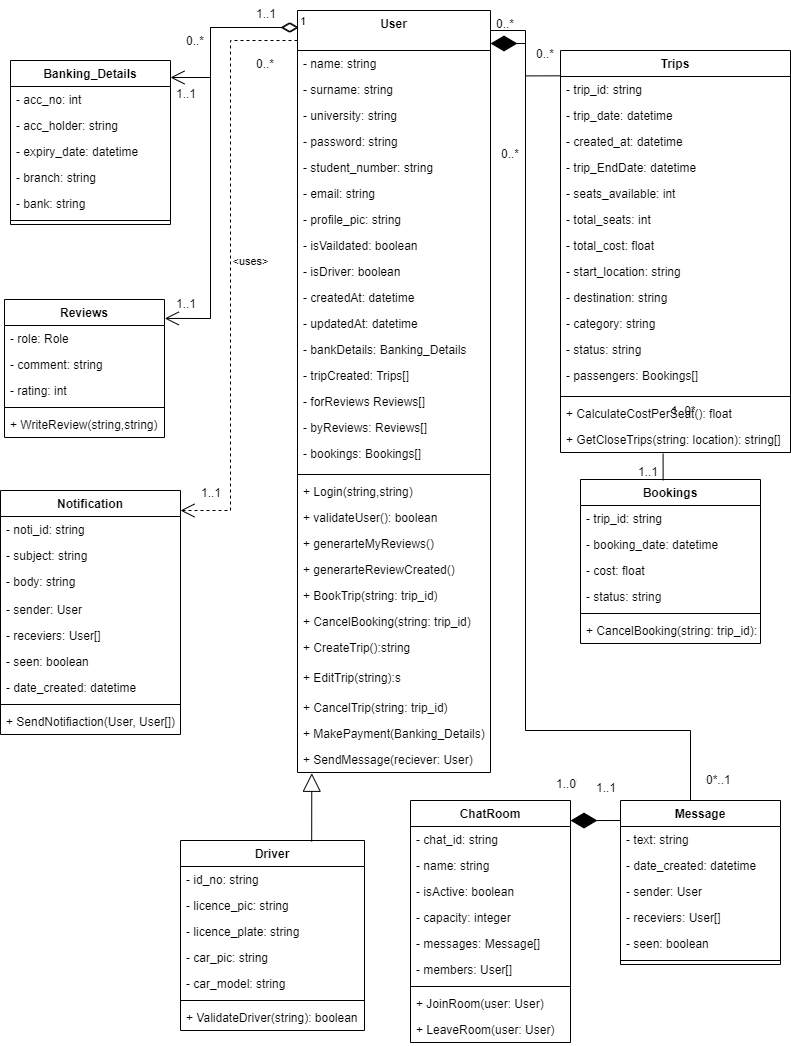
\includegraphics[scale=0.45]{images/Carpool_Class_Diagram.drawio.png}
            \caption{Carpool Class Diagram}
            \label{fig:ClassDiagram}
            
        \end{figure}
   \newpage     
        \subsection{Analysis of Class Diagram}
        
    \subsubsection{User}
        This table stores all the necessary information of the user. A user can be either a passenger, driver or both.

    \subsubsection{Banking\_Details}
       This table is responsible for storing the user’s banking details. The user can only have one bank account, and bank account can belong to only one user.
        
    \subsubsection{Reviews}
        This table stores the reviews that users leave on other user’s profiles. The role attribute refers to Driver or Passenger. A user can leave many different reviews on many different profiles, however a review can only be created by one user.
                
    
       \subsubsection{Notification table}
        This table stores all notifications that were sent either by a driver or an admin user. A notification can be sent to multiple users at the same time, however a notification can only be sent by one person.


       \subsubsection{Trips}
        This table is responsible for storing the trips that the user(driver) has created. It stores the necessary information about the trip that has been created. A user (driver) can post/ create many different trips however only one user can post/create a trip.
       
    
       \subsubsection{Booking}
        This table is responsible for storing the bookings that have been made by the user(passenger). Booking occurs when a user(passenger) requests an available seat on a trip that has been created. The booking is only confirmed once the driver has accepted their request. A user can have many bookings on many trips, however a booking can only relate to one user. A trip can have many bookings (since more then one passenger can join a trip), but a booking can only belong to one trip.
        
       \subsubsection{ChatRoom}
        This is responsible for storing information relating to a chatroom. A chatroom is created when the user confirms a booking. The chatroom allows all users that partake in the trip to send messages to one another in a central location, instead of sending messages to each user individually. A user can belong to many chatrooms, and a chatroom can have many different users.

    
      \subsubsection{Message}
        This is the actual message that is sent on the chatroom. This table stores all necessary information about the message sent as well as who sent the message, and who receives the message. A message can belong to only one chatroom, but a chatroom can consists of many different messages. A user can create many different messages, but a message can only be created/sent by one user.

    \subsubsection{Driver}
    Since a user can be both a driver and a passenger, the driver table stores all information relating to the driver. This ensures that the User table does not have null fields, since if a user is a passenger they won’t need to enter their car model and a picture of their license.
         
\newpage
\section{Subsystems}

     \subsection{User:}
                \subsubsection{Use Cases}
                  The User subsystem manages all operations where a User needs to interact with the other subsystems:
                  
                    \begin{figure}[H]
                    
                        \centering
                        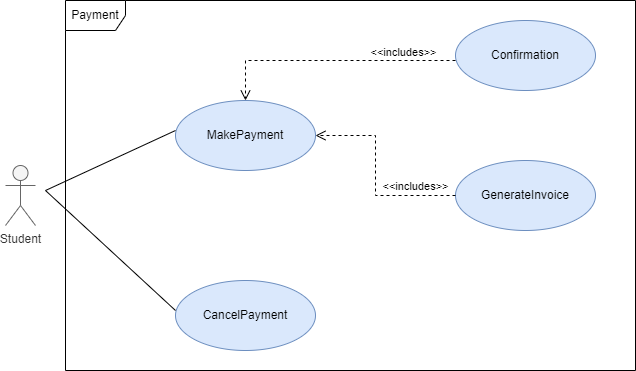
\includegraphics[width=15cm]{images/Payment UseCase.drawio.png}
                        \caption{User Use Cases}
                        \label{fig:User UseCases}
                        
                    \end{figure}
            
             \begin{enumerate}[label=U1.\arabic*]
    
                \item Login:\\
                	The user will be asked to enter their username (student email address) and password in order to access the functionality of the application. If the user enters the correct credentials, they will be issued with a token which will be stores on their local storage.

                \item Register:\\
                	In order to access the functionality of this application, the user has to have an account. The user can create an account by entering their, name, surname, university, email, student number and profile picture

                \item ForgotPassword:\\
                	A link will be sent to the user’s email address, when the user clicks on the link, they will be directed to a website whereby they will be allowed to change their password in a secure manner. The database will be updated with this new password, the userid, and new password will be passed into this function.
                	
                \item EditProfile: \\
                    The user will be provided with the opportunity to edit their profie, such as their name, surname, and profile picture. The userid as well as what information the user would like to edit will be passed into this function.
                    
                \item EditPaymentMethod:\\
                    The user will be provided with the opportunity to change their banking details and their payment method (cash or card). The userid as well as the updated banking details/ payment method will be passed into this function.
                    
                \item VerifyStudent:\\
                    The admin user will verify newly registered students through their email address. The function will take in the student’s email address as a parameter, and return a Boolean value (based on if the user is valid or not). This verification ensures that the user is a student at a recognized university in South Africa.                
                    
                \item AddAdmin:\\
                	The admin user is able to add new admin users to the database. This function will take in the admin user’s name, surname, email, student number and profile picture. A new user will be created in the database.
                	
                \item DeleteUser: \\
                    The admin user is able to delete/ remove any user from the Carpool application. The userid of the user who should be removed should be passed into this function. The user will be removed from the database.
                    
                    \end{enumerate}
                    
\newpage
                \subsection{Payment:}
                \subsubsection{Use Cases}
                  The Payment subsystem is responsible for ensuring that the user is able to make secure payments via the application. This could be done using payFast:
                    
                    \begin{figure}[H]
                    
                        \centering
                        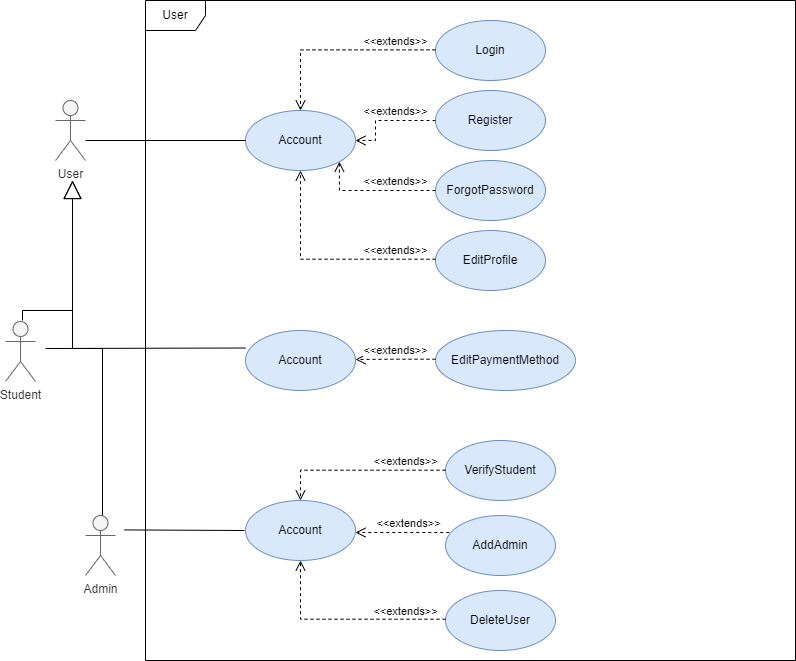
\includegraphics[width=15cm]{images/User Usecase.drawio.png}
                        \caption{Payment Use Cases}
                        \label{fig:User UseCases}
                        
                    \end{figure}
                    
            \subsubsection{Service Contract}
             \begin{enumerate}[label=U1.\arabic*]

                \item MakePayment:\\
                When a user would like to make payment for their booking, this function will be called. The function will take in as parameters : account holder, account number, password, OTP, amount due)

                \item Confirmation:\\
                	This use case is responsible for sending a confirmation email to the user once the payment is reflected as successful. The function takes in the userid as a parameter.

                \item GenerateInvoice:\\
                This use case is responsible for generating an invoice that will be emailed along with the confirmation to the user. This is only done when the payment is successful.
                	
                \item CancelPayment: \\
            The user is provided with the opportunity to cancel their payment. The money that they paid will be refunded to them.
               
                
            \end{enumerate}
            
            \vspace{1cm}
                \subsection{Reviews:}
                \subsubsection{Use Cases}
                   The review subsystem allows user’s to rate and review other users in the application. Driver’s can rate passengers and passengers can rate drivers. This rating allows users to gain insight on how their driver/passenger conducts themselves on trips.
                    
                    \begin{figure}[H]
                    
                        \centering
                        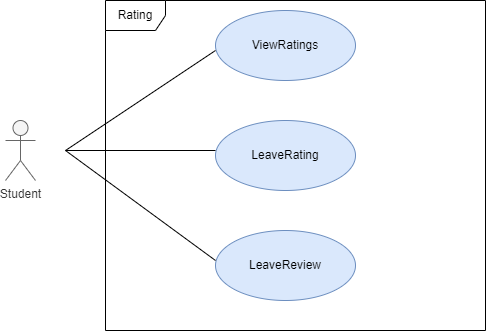
\includegraphics[]{images/Rating Usecase.drawio.png}
                        \caption{Reviews Use Cases}
                        \label{fig:User UseCases}
                        
                    \end{figure}
         \newpage           
                \subsubsection{Service Contract}
            
             \begin{enumerate}[label=U1.\arabic*]

                \item ViewRatings:\\
                    The user is able to view all their ratings, These are ratings that have been created by other users. This function will return a list of all the user’s ratings, both positive and negative.\\

                \item LeaveRating:\\
                	This function returns a list of notifications that the user has received. The user is able to view all their notifications on one page\\

                \item LeaveReview:\\
                    The user is able to rate other users via this use case. This function takes in the userid of the user who wants to leave the rating, the userid of the user whom the rating is about, and the rating.\\
                	
                \item NotifyUserWhenTripFullyBooked: \\
                    The user is able to review other users via this use case. This function takes in the userid of the user who wants to leave the review, the userid of the user whom the review is about, and the review. Ratings are integer/ stars and reviews are usually longer sentence.\\
               
            \end{enumerate}
            
    \newpage
                    \subsection{Notifications:}
                \subsubsection{Use Cases}
                  The notification subsystem allows admin to send notifications to users when their trips are fully booked and when they have been validated. The notification subsystem also allows users to send notifications to other users in the trip reminding them about the trip.
                  \vspace{1cm}
                    
                    \begin{figure}[H]
                    
                        \centering
                        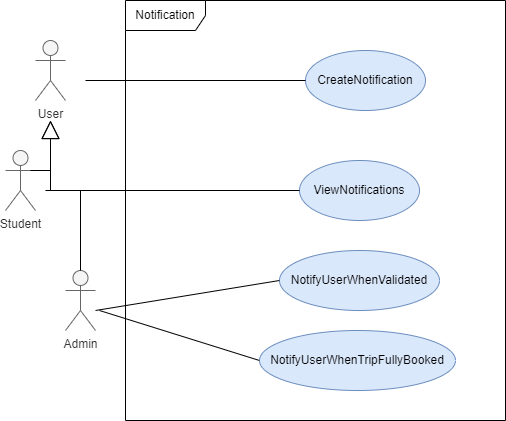
\includegraphics[]{images/Notification Usecase.drawio.png}
                        \caption{Notifications Use Cases}
                        \label{fig:User UseCases}
                        
                    \end{figure}
   \newpage                 
                \subsubsection{Service Contract}
            
             \begin{enumerate}[label=U1.\arabic*]

                \item CreateNotification:\\
                    This function will allow users to create notifications, passed as a parameter will be the context of the notification as well as the user/users that one would like to send the notification to.\\

                \item ViewNotifications:\\
                	This function returns a list of notifications that the user has received. The user is able to view all their notifications on one page\\

                \item NotifyUserWhenValidated:\\
                    The admin users will make use of this function once they have completed validating a user’s email address or drivers license. This will make the users aware of their validation status and they can then start using the application as soon as possible. The parameters will be the userid’s of those users who have been validated successfully.\\
                	
                \item NotifyUserWhenTripFullyBooked: \\
                    This allows drivers and passengers to know when their trip has been fully booked. Passengers will pay the minimum price for a seat, and driver won’t have to worry about looking for more people to carpool with. This will take in all the users that belong to the fully booked trip as a parameter.\\
               
     \end{enumerate}
\newpage
                \subsection{Trips:}
                \subsubsection{Use Cases}
                    The trips subsystem is where the core functionality of the application occurs, users are able to browse, book and create trips in this subsystem
                    
                    \begin{figure}[H]
                    
                        \centering
                        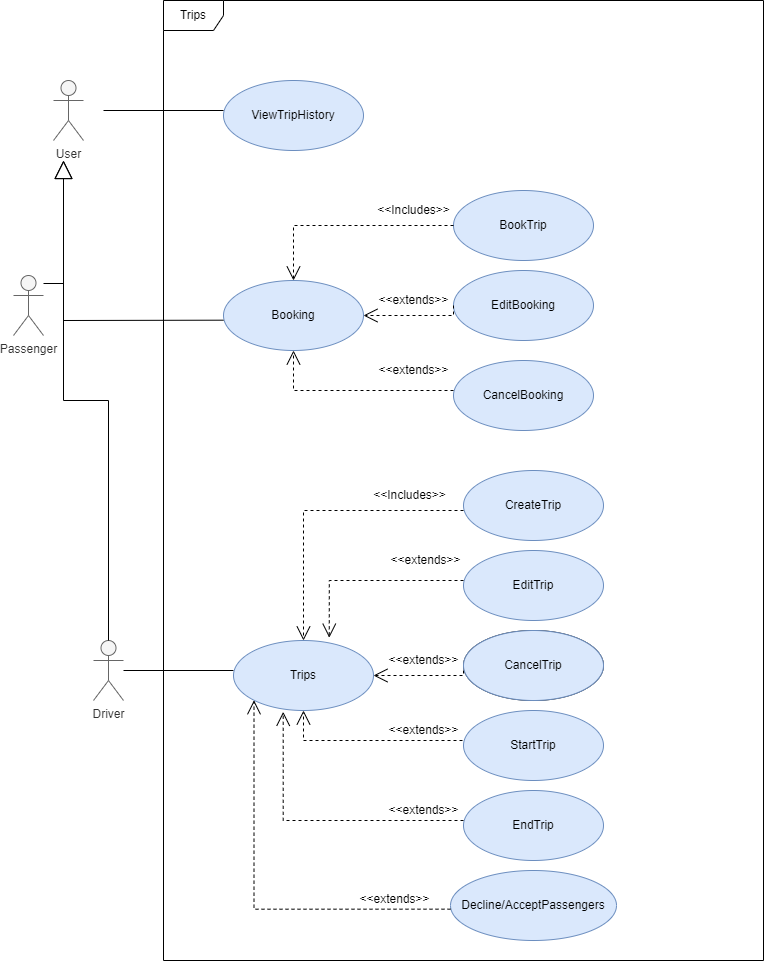
\includegraphics[width = 15cm]{images/Trips Usecase.drawio.png}
                        \caption{Trips Use Cases}
                        \label{fig:User UseCases}
                        
                    \end{figure}
         \newpage           
                \subsubsection{Service Contract}
            
             \begin{enumerate}[label=U1.\arabic*]

                \item ViewTripHistory:\\
                This allows the user to view the previous trips that they have booked or that they have created. The developers will also use this this function to recommend trips to passengers.\\

                \item BookTrip:\\
                Users will be provided with the functionality to book a trip that has available seats. Booking a trip can be split into two functions: 
                Requesting a Trip – The user will first have to request to be apart of said trip, the user will have to wait for confirmation from the driver of the trip.
                Confirmed Trip – Once the trip has been confirmed, the user will receive a notification about this confirmation and will be able to edit/cancel their booking.\\

                \item EditBooking:\\
                The passenger will be able to edit their booking, by increasing the number of seats that they would like to book, or their start location.\\
                	
                \item CancelBooking: \\
                The passenger will be provided with the opportunity to cancel their booking, the driver will be notified about this confirmation. If payment has been made, then the passenger will be refunded.\\
                    
                \item CreateTrip:\\
                Drivers can create a  trip, when creating the trip they need to include : date of trip, seats available, price per seat, starting location and destination of the trip. The database will then record all this information and this trip will be displayed on the view Trip page.\\
                    
                \item EditTrip:\\
                Drivers can then edit the trips they created, by changing the information that they have entered(date of trip, seats available, price per seat, starting location and destination of the trip). They can also deny previously confirmed passengers of joining the trip. The database will be updated accordingly.\\

                \item CancelTrip:\\
                A driver can cancel the trips that they have created, when they cancel the trip. Passengers who were supposed to be apart of the trip will be notified. The trip’s information will be removed from the database and users will no longer be able to join the trip since it does not exist anymore.\\
                	
                \item StartTrip: \\
                When the driver begin their trip (ready to pick up fellow passengers), they need to start the trip, when they begin their trip, the passengers will be notified that their driver is on their way to pick them up.\\
                
                \item EndTrip:\\
                Once the driver has arrived at the desired destination with the required passengers, the driver will be asked to end the trip. This is to ensure that the trip has been completed successfully and participants of the trip have arrived safely of their destination. The trip will then be categorized  as completed in the database.\\

                \item Decline/Accept Passengers:\\
                The driver will be allowed to accept and decline passengers that would like to join their trip. This allows the driver to ensure that they are travelling with people they are comfortable with. Before accepting/ declining the passenger, the user will be prompted to view the passengers profile, ensuring that the driver makes and informed decision.\\
                	
            \end{enumerate}

\newpage
                \subsection{Searching :}
                \subsubsection{Use Cases}
                The searching subsystem allows users to browse for trips based on many different criteria’s and filters. A list of trips that match the criteria will be displayed to the user.
                    
                    \begin{figure}[H]
                    
                        \centering
                        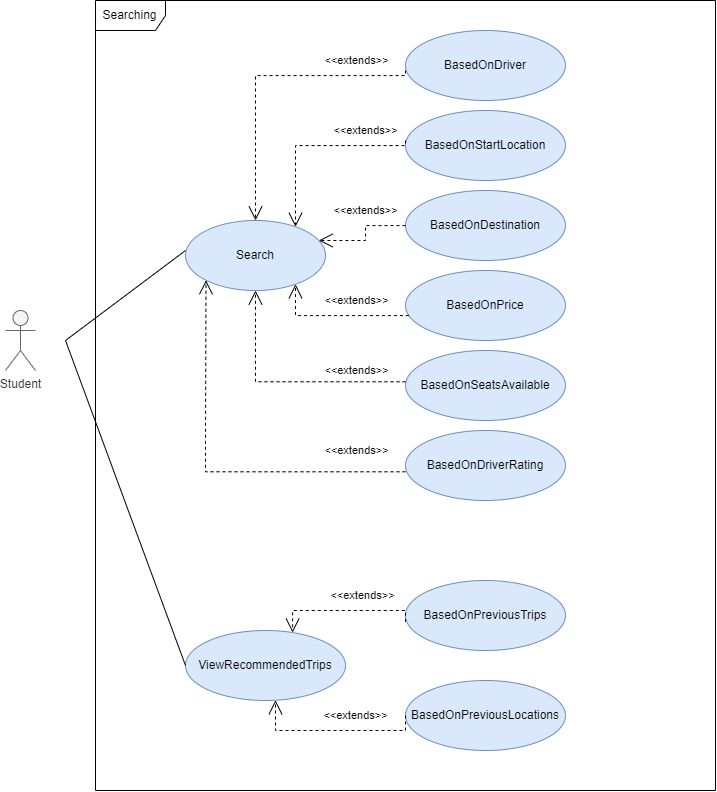
\includegraphics[width = 15cm]{images/SearchingUseCase.drawio.png}
                        \caption{Searching Use Cases}
                        \label{fig:User UseCases}
                        
                    \end{figure}
         \newpage           
                \subsubsection{Service Contract}
            
             \begin{enumerate}[label=U1.\arabic*]

                \item BasedOnDriver:\\
                Passengers will be provided with the opportunity to search for a trip based on the drivers name. The name of the driver will be passed as a parameter into this function. Trips that the driver has currently posted will then be displayed to the passenger.\\
                 

                \item BasedOnStartLocation:\\
                Passengers will be provided with the opportunity to search for a trip based on their start location. Their start location  will be passed as a parameter into this function. Trips that are near their start location will be displayed to the user.\\

                \item BasedOnDestination:\\
                Passengers will be provided with the opportunity to search for a trip based on their end  location. Their end  location  will be passed as a parameter into this function. Trips that are near their end location will be displayed to the user.\\
                U6.2 
	
                \item BasedonPrice: \\
                Passengers will be provided with the opportunity to search for a trip based on the price of the available seat. Trips will then be displayed to the user from lowest seat cost to highest seat cost, or vice versa depending on the passenger’s needs.\\
                    
                \item BasedOnSeatsAviailable:\\
                Passengers will be provided with the opportunity to search for a trip based on the number of seats available (Trips that have more seats will be displayed first or trips that have one seat left will be displayed first. Trips that match this criteria will then be displayed to the user. \\
                    
                \item BasedOnDriversRating:\\
                Passengers will be provided with the opportunity to search for a trip based the rating of the drivers. Trips that have drivers will high ratings will displayed at the top of the page, and drivers with low ratings will be displayed towards the end of the page.\\

                \item BasedOnPreviousTrips:\\
                Admin will use this function to view the user’s previous trips, and recommend trips to the user based on their previous trips. Information like the driver, driver’s rating and cost can be used to find a trip that the passenger will most likely join. The trip will be added to an array.\\
                	
                \item BasedOnPreviousLocations: \\
                Admin will use this function to view the user’s previous trip, and based on their previous locations recommend a trip to them. The function scans through all trips that have been posted in the database, and matches the users  previous locations to locations in the database. If there is a match, then the trip is added to an array..\\
                
                \item Search:\\
                Passengers will be provided with the opportunity to search for a trip based on different criteria. The criteria will then be passed as a parameter to the specific search function. Trips that meet the criteria will be displayed to the user.\\

                \item ViewRecommendedTrips:\\
                The user will be able to view all the trips that have been recommended to them by the system. These recommended trips will be based on their previous trips(previous location, cost, driver). \\
                	
            \end{enumerate}
\newpage
                \subsection{Chat :}
                \subsubsection{Use Cases}
                The chat subsystem allows the user to send and receive messages from other user within the carpool application. Users are added to chatrooms when their trips are confirmed, and the users part of that trip are able to talk to one another in a central location.
                    
                    \begin{figure}[H]
                    
                        \centering
                        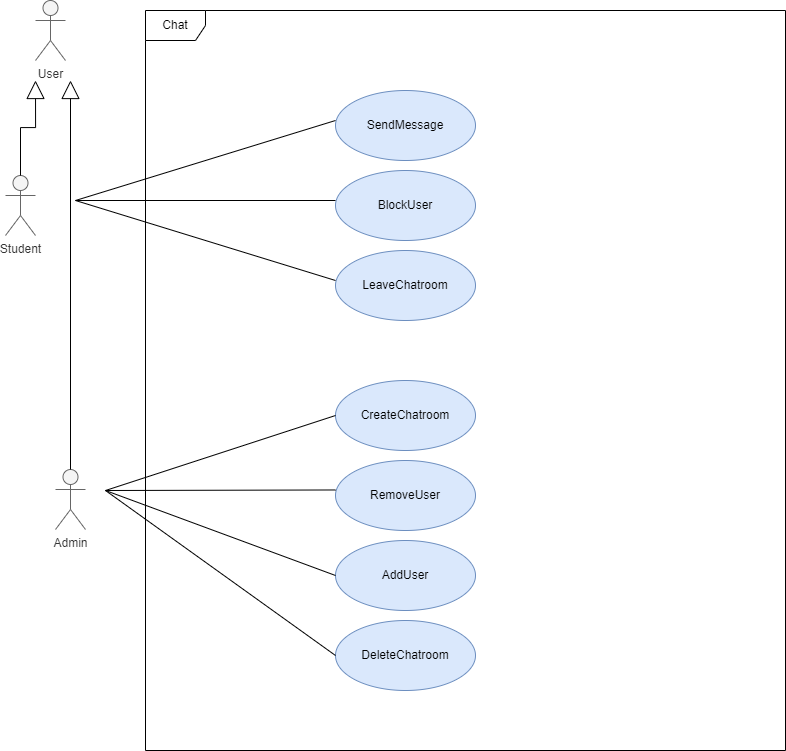
\includegraphics[width = 15cm]{images/Chat Usecase.drawio.png}
                        \caption{Chat Use Cases}
                        \label{fig:User UseCases}
                        
                    \end{figure}
         \newpage           
                \subsubsection{Service Contract}
            
             \begin{enumerate}[label=U1.\arabic*]

                \item SendMessage:\\
                User will be allowed to send messages on the group chat, The content of the message as well as the sender and receivers of the message will be passed into the function as parameters. The message will  then be stored in the database and displayed in the chat room for that particular trip.\\
                 

                \item BlockUser:\\
                Users will be provided with the opportunity to block another user, they will no longer be able to receive messages from that passenger, nor will they be able to join a trip with a user that they have blocked. The userid of the blocked user, and the userid of the user who wants to block someone will be passed as a parameter in the function. The system will then ensure that the user does not receive or join trips with said blocked user.\\
        
               \item LeaveChatroom:\\
                User’s will be provided with the opportunity to leave the chatroom that has been created for a specific trip. The userid of the user that wants to leave the trip will be passed as a parameter into the function. The user will then be removed from the chatroom row in the database. The user will no longer receive messages from said chatroom.\\
	
                \item CreateChatroom: \\
                When a driver creates a trip, a chatroom is automatically created by the system. Every time a passenger is confirmed to be apart of the trip, they are added to the chatroom.\\
                    
                \item RemoveUser:\\
                Admin is allowed to remove a passenger from the chatroom, the userid of the passenger that Admin wants to remove will be passed as a parameter into the function. The user is then removed from the chatroom row in the database. The user is no longer a participant of the chatroom and can no longer receive messages from that chatroom.\\
                    
                \item AddUser:\\
                Admin is allowed to add a user to the chatroom, the userid of the passenger Admin wants to add to the chatroom will be passed as a parameter. When a passenger is confirmed to be a participant in the trip, this function will be called so that the user can be apart of the chatroom for that trip. The user is added to the chatroom row in the database. The user can now receive and send messages via the chatroom.\\

                \item DeleteChatroom:\\
                Admin can delete the chatroom, the id of the chatroom is passed through this function. The chatroom with that particular id is removed from the chatroom table in the database. This function is called automatically by the system .when the trip has been complete.\\
    \end{enumerate}
    \newpage
    \section{Traceability Matrix}


\begin{table}[H]
    \centering
        \begin{tabular}{|l|l|l|c|c|c|c|c|c|}
        \hline
    
            \multicolumn{9}{|c|}{Subsystems} \\ \hline
            &      & 7.1  & 7.2   & 7.3 & 7.4 & 7.5 & 7.6  &7.7 \\ \hline
        \multirow{22}{*}{Requirements}
        & R1    &   X   &       &      &    &      &   &    \\ \cline{2-9} 
        & R2    &   X   &       &      &    &      &   &    \\ \cline{2-9} 
        & R3    &   X   &       &      &    &      &   &    \\ \cline{2-9} 
        & R4    &       &       &      &    &   X  &   &     \\ \cline{2-9}
        & R5    &       &       &      &    &      & X &    \\ \cline{2-9}
        & R6    &       &       &      &    &   X  &   &    \\ \cline{2-9}
        & R7    &       &       &      &    &      & X &    \\ \cline{2-9}
        & R8    &       &   X   &      &    &      &   &    \\ \cline{2-9}
        & R9    &       &       &   X  &    &      &   &    \\ \cline{2-9}
        & R10   &       &       &      &    &      & X &    \\ \cline{2-9}
        & R11   &       &       &      &    &      &   &  X  \\ \cline{2-9}
        & R12   &       &       &      &    &      & X &     \\ \cline{2-9}
        & R13   &       &       &      &    &      & X &     \\ \cline{2-9}
        & R14   &   X   &       &      &    &      &   &    \\ \cline{2-9}
        & R15   &       &       &      &  X &      &   &    \\ \cline{2-9}
        & R5.1  &   X   &       &      &    &      &   &    \\ \cline{2-9}
        & R5.2  &       &       &      &    &      &   &  X  \\ \cline{2-9}
        & R5.3  &       &       &  X   &    &      &   &    \\ \cline{2-9}
        & R5.4  &       &   X   &      &    &      &   &    \\ \cline{2-9}
        & R5.5  &       &       &      &    &   X  &   &    \\ \cline{2-9}
        & R5.6  &       &       &      &    &      &   &    \\ \cline{1-9}
                                    
        \end{tabular}
        \vspace{1cm}
    \caption{Transability matrix with requirements numbers as rows and the sub-systems as columns}
    \label{table:Could-haveRequirementsTraceabilityMatrix}
\end{table}

\begin{table}[H]
    \centering
        \begin{tabular}{|l|l|l|c|c|c|c|c|c|c|c|c|c|c|c|c|c|c|}
        \hline
    
            \multicolumn{17}{|c|}{Requirements} \\ \hline
            &  & R1  & R2   & R3 & R4 & R5 & R6 & R7 &R8 & R9 & R10 & R11 & R12 & R13 & R14 & R15    \\ \hline
        \multirow{29}{*}{Use cases}

        & U1.1 &    &  X     &     &   &   &   &   &   &   &   &   &   &   & X    &  \\ \cline{2-17}
        & U1.2 & X  &       &      &   &   &   &   &   &   &   &   &   &   &    &  \\ \cline{2-17}    
        & U1.3 &    &   X    &     &   &   &   &   &   &   &   &   &   &   &    &  \\ \cline{2-17}    
        & U1.4 & X  &       &      &   &   &   &   &   &   &   &   &   &   &    &  \\ \cline{2-17}    
        & U1.5 & X  &       &      &   &   &   &   &   &   &   &   &   &   &    &  \\ \cline{2-17}    
        & U1.6 &    &        &  X  &   &   &   &   &   &   &   &   &   &   &    &  \\ \cline{2-17}    
        & U1.7 & X  &       &      &   &   &   &   &   &   &   &   &   &   &    &  \\ \cline{2-17}    
        & U1.8 & X  &       &      &   &   &   &   &   &   &   &   &   &   &    &  \\ \cline{2-17}    
        & U2.1 &    &       &      &   &   &   &   &  X &   &   &   &   &   &    &  \\ \cline{2-17}    
        & U2.2 &    &       &      &   &   &   &   &  X &   &   &   &   &   &    &  \\ \cline{2-17}    
        & U2.3 &    &       &      &   &   &   &   &  X &   &   &   &   &   &    &  \\ \cline{2-17}    
        & U2.4 &    &       &      &   &   &   &   &  X &   &   &   &   &   &    &  \\ \cline{2-17}    
        & U3.1 &    &       &      &   &   &   &   &   & X  &   &   &   &   &    &  \\ \cline{2-17}    
        & U3.2 &    &       &      &   &   &   &   &   & X  &   &   &   &   &    &  \\ \cline{2-17}    
        & U3.3 &    &       &      &   &   &   &   &   & X  &   &   &   &   &    &  \\ \cline{2-17}    
        & U4.1 &    &       &      &   &   &   &   &   &   &   &   &   &   &    & X \\ \cline{2-17}    
        & U4.2 &    &       &      &   &   &   &   &   &   &   &   &   &   &    & X \\ \cline{2-17}    
        & U4.3 &    &       &      &   &   &   &   &   &   &   &   &   &   &    & X \\ \cline{2-17}    
        & U4.4 &    &       &      &   &   &   &   &   &   &   &   &   &   &    & X \\ \cline{2-17}    
        & U5.1 &    &       &      &   & X  &   &   &   &   &   &   &   &   &    &  \\ \cline{2-17}    
        & U5.2 &    &       &      &   &   & X  &   &   &   &   &   &   &   &    &  \\ \cline{2-17}    
        & U5.3 &    &       &      & X  &   &   &   &   &   &   &   &   &   &    &  \\ \cline{2-17}    
        & U5.4 &    &       &      & X  &   &   &   &   &   &   &   &   &   &    &  \\ \cline{2-17}    
        & U5.5 &    &       &      & X  &   &   &   &   &   &   &   &   &   &    &  \\ \cline{2-17}    
        & U5.6 &    &       &      & X  &   &   &   &   &   &   &   &   &   &    &  \\ \cline{2-17}    
        & U5.7 &    &       &      & X  &   &   &   &   &   &   &   &   &   &    &  \\ \cline{2-17}    
        & U5.8 &    &       &      & X  &   &   &   &   &   &   &   &   &   &    &  \\ \cline{2-17}    
        & U5.9 &    &       &      & X  &   &   &   &   &   &   &   &   &   &    &  \\ \cline{2-17}    
        & U5.10 &   &       &      & X  &   &   &   &   &   &   &   &   &   &    &  \\ \cline{2-17}    
        & U6.1 &    &       &      &   &   &   &  X &   &   &   &   &   &   &    &  \\ \cline{2-17}    
        & U6.2 &    &       &      &   &   &   &  X &   &   &   &   & X &   &    &  \\ \cline{2-17}    
        & U6.3 &    &       &      &   &   &   &  X &   &   &   &   & X  &   &    &  \\ \cline{2-17}    
        & U6.4 &    &       &      &   &   &   &  X &   &   &   &   &   &   &    &  \\ \cline{2-17}    
        & U6.5 &    &       &      &   &   &   &  X &   &   &   &   &   &   &    &  \\ \cline{2-17}    
        & U6.6 &    &       &      &   &   &   &  X &   &   &   &   &   &   &    &  \\ \cline{2-17}    
        & U6.7 &    &       &      &   &   &   &   &   &   &   &   &   & X  &    &  \\ \cline{2-17}    
        & U6.8 &    &       &      &   &   &   &   &   &   &   &   &   & X  &    &  \\ \cline{2-17}    
        & U6.9 &    &       &      &   &   &   & X  &   &   &   &   &   &   &    &  \\ \cline{2-17}    
        & U6.10 &   &       &      &   &   &   &   &   &   & X  &   &   &   &    &  \\ \cline{1-17}    
  

   \end{tabular}
   \vspace{0.2cm}
    \caption{Transability matrix with use cases as rows and requirements as columns}
    \label{table:ContinuedCould-haveRequirementsTraceabilityMatrix}
\end{table}
\newpage
\begin{table}[H]
    \centering
        \begin{tabular}{|l|l|l|c|c|c|c|c|c|c|c|c|c|c|c|c|c|c|}
        \hline
    
            \multicolumn{17}{|c|}{Requirements} \\ \hline
            &  & R1  & R2   & R3 & R4 & R5 & R6 & R7 &R8 & R9 & R10 & R11 & R12 & R13 & R14 & R15    \\ \hline
        \multirow{7}{*}{Use cases}
        
        & U7.1 &    &       &      &   &   &   &   &   &   &   & X  &   &   &    &  \\ \cline{2-17}    
        & U7.2 &    &       &      &   &   &   &   &   &   &   & X  &   &   &    &  \\ \cline{2-17}    
        & U7.3 &    &       &      &   &   &   &   &   &   &   & X  &   &   &    &  \\ \cline{2-17}    
        & U7.4 &    &       &      &   &   &   &   &   &   &   & X  &   &   &    &  \\ \cline{2-17}    
        & U7.5 &    &       &      &   &   &   &   &   &   &   & X  &   &   &    &  \\ \cline{2-17}    
        & U7.6 &    &       &      &   &   &   &   &   &   &   & X  &   &   &    &  \\ \cline{2-17}    
        & U7.7 &    &       &      &   &   &   &   &   &   &   & X  &   &   &    &  \\ \cline{1-17}    
        
   \end{tabular}
   \vspace{1cm}
    \caption{Transability matrix with use cases as rows and requirements as columns}
    \label{table:ContinuedCould-haveRequirementsTraceabilityMatrix}
\end{table}

\newpage
\section{KO}

    \end{document}